\section{Architecture du projet: Diagrammes des modules et des classes}
Composants principaux :
\begin{enumerate}
    \item Cellule (Cellule.java) :
    \item Grille (Grilles.java) 
    \item Règles (Regle.java) 
    \item Interface Graphique :
    \item Structures de Données 
    \begin{enumerate}
        \item Enum Etat
    \end{enumerate} 

\end{enumerate}

\newpage
Voici sur la figure au dessus le diagramme de classe de notre projet, sur lequel figure les différents paquetages et ses interactions avec les autres paquetages.

    \begin{figure}
\begin{center}
        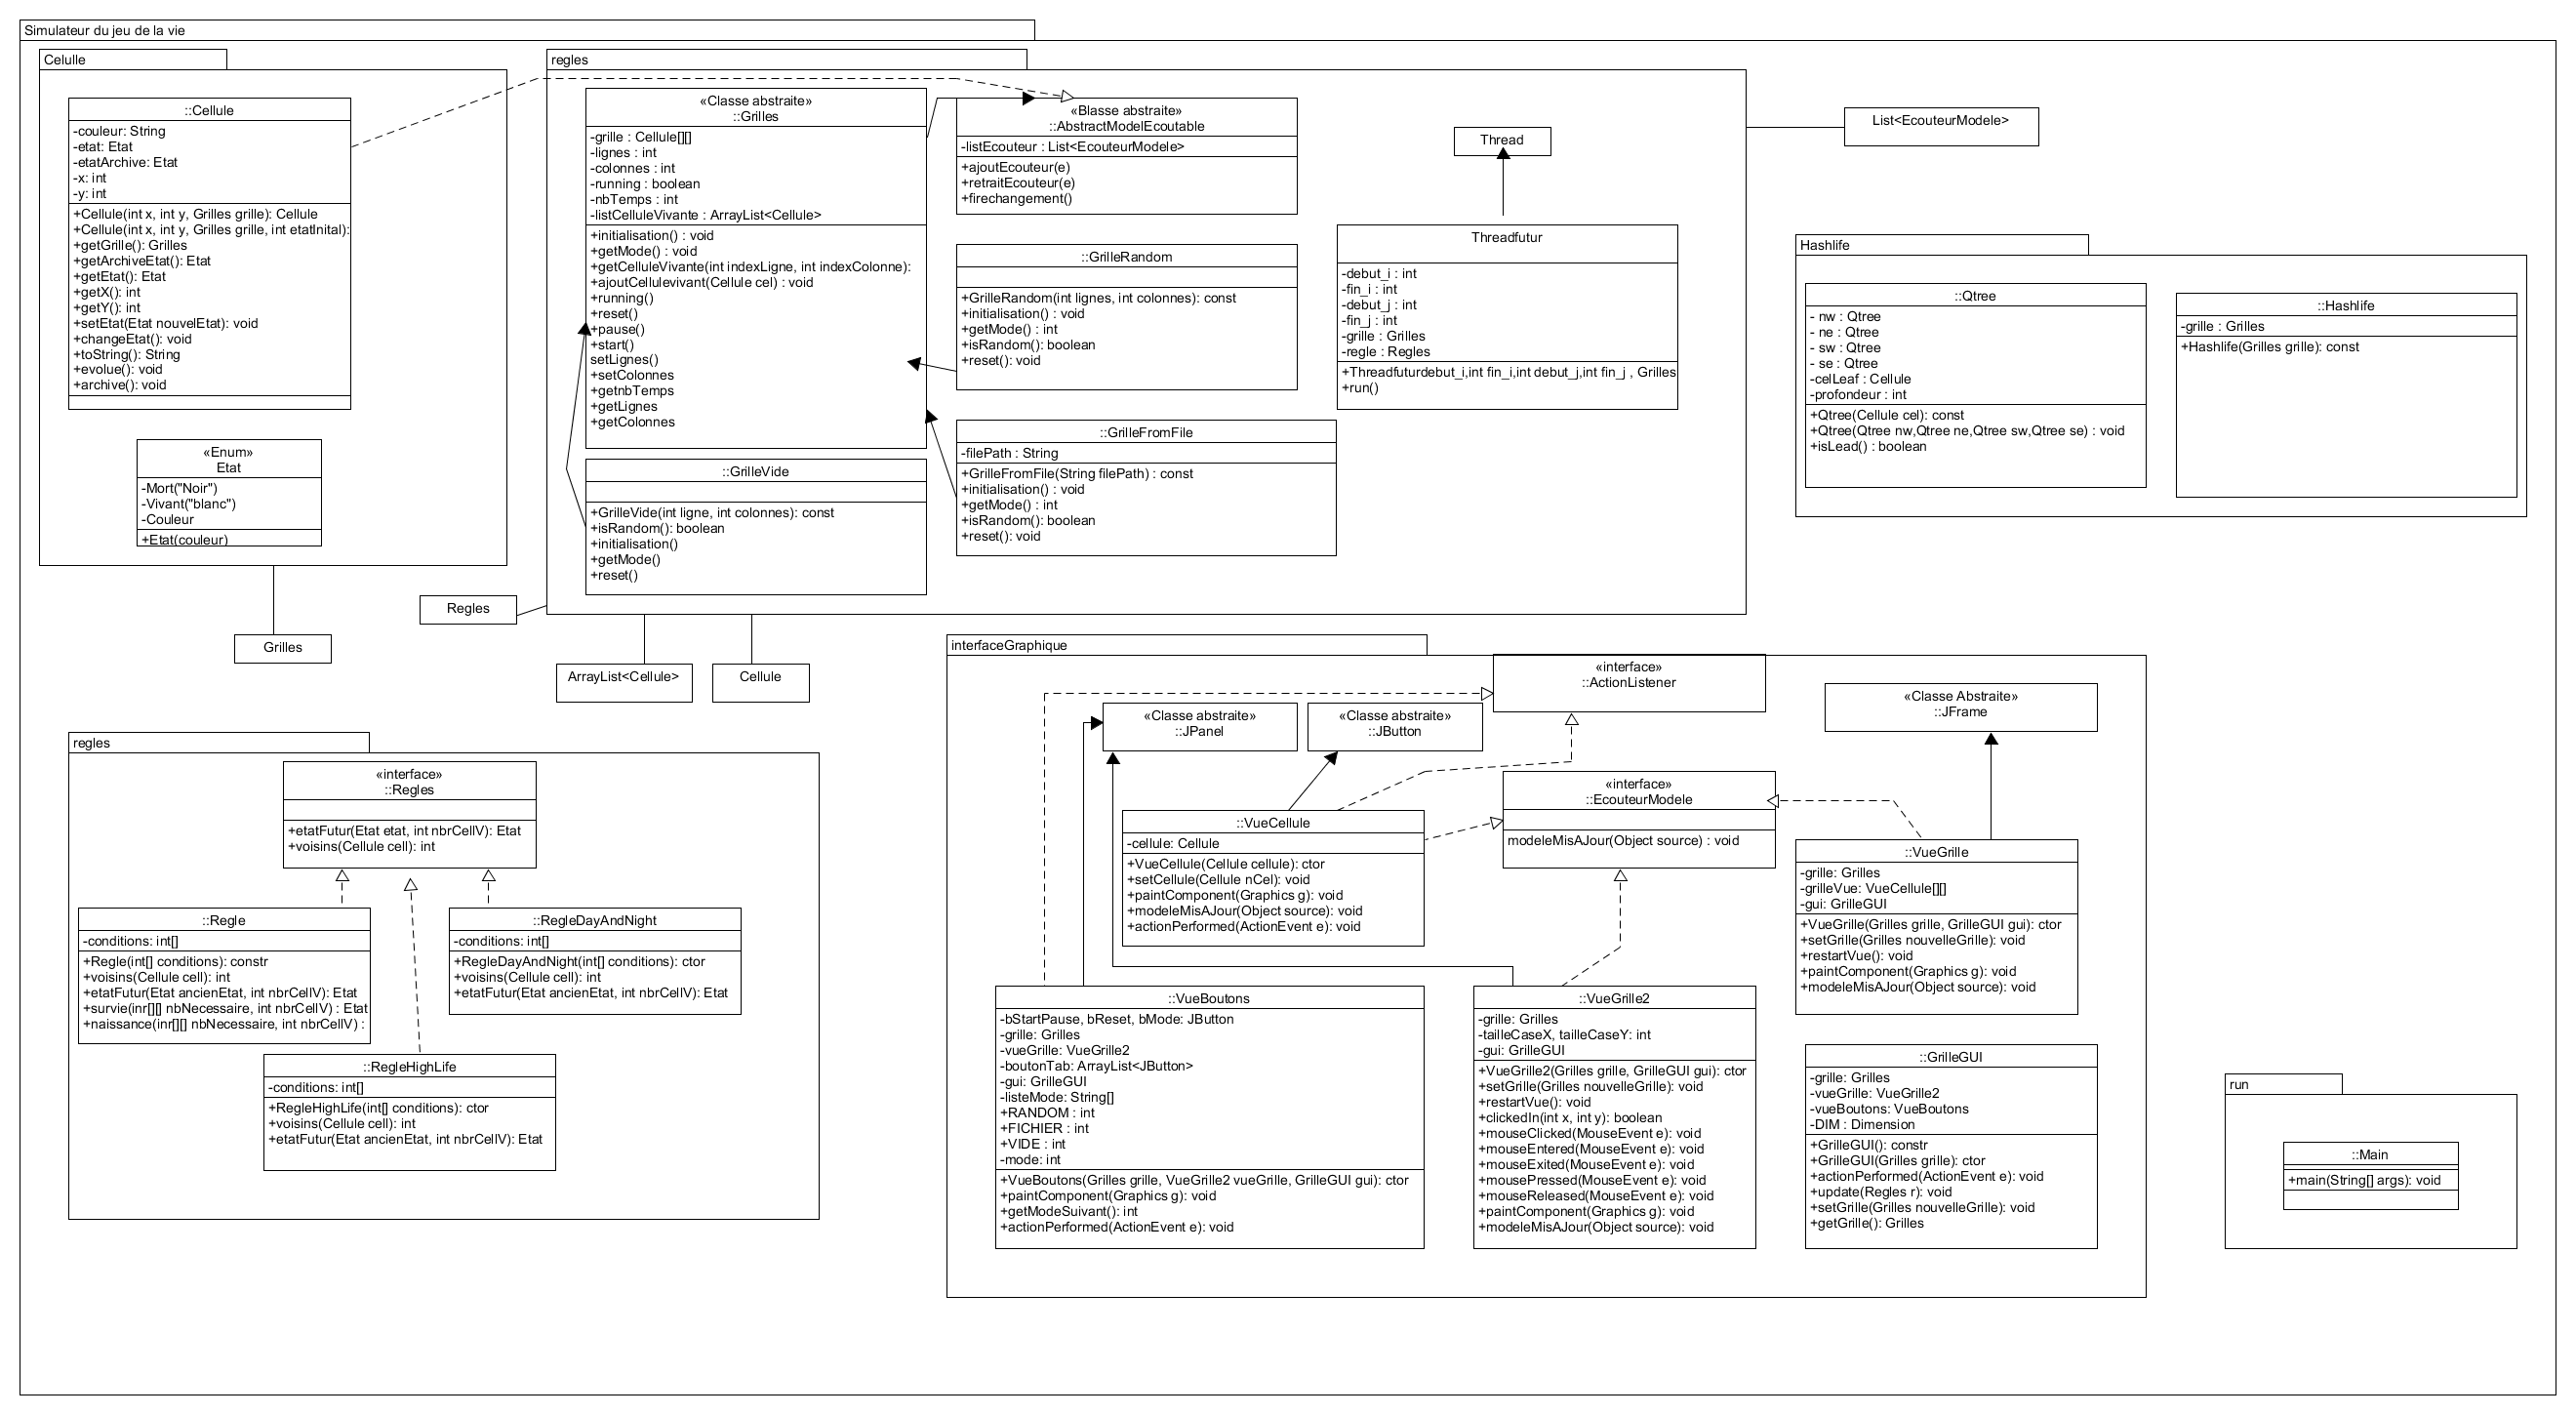
\includegraphics[width=120mm,scale=0.5]{figures/uml.png}
    \captionof{figure}{Diagramme de classe}
\end{center}
\end{figure}


\subsection{Chaînes de traitement (comment les classes interagissent et pourquoi)}

Interaction entre Grilles et Cellule :
Comme expliqué precedemment,\ref{exp} la classe Grilles représente la grille de cellules, tandis que la classe Cellule représente chaque cellule individuelle dans cette grille.
Pendant l'initialisation de la grille, Grilles crée un tableau 2D de Cellule pour représenter toutes les cellules de la grille.
Chaque cellule (Cellule) contient des informations sur son état (vivant ou mort via un Enum) et ses coordonnées (x et y).

Grilles utilise setEtat() pour modifier l'état d'une cellule en fonction des règles du jeu de la vie.

Interaction entre Regles et Grille:
La méthode futur(Regles r) de la classe Grilles est responsable de calculer l'état futur de chaque cellule en fonction des règles pré-definnies.

Pour chaque cellule dans la grille, Grilles utilise Regles.voisins() pour estimer d'abord le nombre de voisins vivants de la cellule puis avec cette info, Grilles utilise ensuite Regles.etatFutur() pour fixer le nouvel état de la cellule (vivant ou mort) à la prochaine génération.


Interaction partie graphique :

Les classes VueGrille et VueGrille2 sont responsables de l'affichage graphique de la grille de cellules.
Elles reçoivent des mises à jour de la grille à partir de modeleMisAJour(Object source) quand y a des changements
Ces vues parcourent le tableau de Cellule pour afficher avec l'itrface graphiqu chaque cellule à l'écran, en utilisant leurs états (Etat.Vivant ou Etat.Mort) pour déterminer la couleur.

Interaction avec l'interface utilisateur (GrilleGUI) :

La classe GrilleGUI agit comme une interface utilisateur pour le jeu.
Elle utilise (VueGrille, VueBoutons) pour afficher la grille et permettre à l'utilisateur d'interagir avec le jeu (start, pause, réinitialiser).
Lorsque l'utilisateur cliques sur les boutons ("Start" ou "Reset"), des événements (ActionEvent) sont lancés, ce qui conduit à des actions comme démarrer ou arrêter la simulation dans la grille (Grilles).
